\section{Non-Maximum Suppression}

Non-Maximum Suppression (NMS) is a technique used to thin out the edges detected in the gradient image, ensuring that only the most significant edges are retained. This step is essential for refining the edge map and removing spurious responses, which helps in accurately identifying the true edges in an image.

Technically, NMS examines the gradient magnitude and direction at each pixel, comparing it with neighboring pixels along the gradient direction. If the current pixel's magnitude is not the maximum, it is suppressed (set to zero); otherwise, it is retained. This ensures that only local maxima are preserved, resulting in a thinned edge map.

In simpler terms, NMS sharpens blurry, thick edges by keeping only the highest points along an edge direction, like tracing an outline with a fine-tipped pen instead of a broad marker.

The process of Non-Maximum Suppression can be broken down into the following steps:

\begin{enumerate}
    \item Compute the gradient direction for each pixel in the gradient image using \autoref{eq:grad-direction}.
    \item For each pixel, compare its gradient magnitude with the magnitudes of the two neighboring pixels along the gradient direction.
    \item If the pixel's magnitude is not the maximum among the three, set it to zero; otherwise, retain its value.
\end{enumerate}


See in \autoref{fig:nms-examples} for an example of how NMS works. The cell enclosed by red-dashed border is the current pixel that is being processed. The two neighboring pixels with black-dashed borders are the pixels that falls in the gradient direction of the current pixel. In \autoref{fig:nms1} the current pixel's gradient direction is $pi$. And in \autoref{fig:nms2} the current pixel's gradient direction is $5pi/4$.
\autoref{fig:nms1} shows the case when the current pixel is a local maximum. In this case, the current pixel is retained. So, no suppression is done. \autoref{fig:nms2} shows the case when the current pixel is not a local maximum. In this case, the current pixel is suppressed. So, the pixel is set to zero.

\begin{figure}
    \centering
    \begin{subfigure}[b]{0.40\textwidth}
        \centering
        \begin{subfigure}[b]{0.40\textwidth}
            \renewcommand\thesubfigure{\alph{subfigure}1}
            \centering
            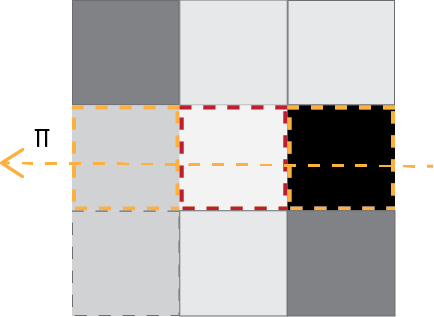
\includegraphics[width=0.9\textwidth]{nms1-before.png}
            \caption{Before NMS}
            \label{fig:nms1-before}
        \end{subfigure}
        \hfill
        \begin{subfigure}[b]{0.40\textwidth}
            \addtocounter{subfigure}{-1}
            \renewcommand\thesubfigure{\alph{subfigure}2}
            \centering
            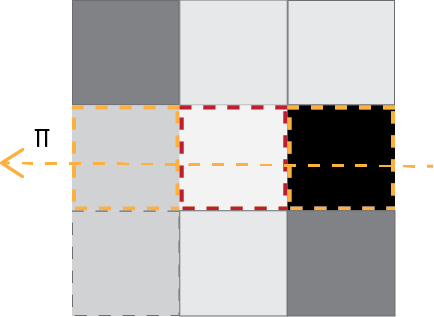
\includegraphics[width=0.9\textwidth]{nms1-after.png}
            \caption{After NMS}
            \label{fig:nms1-after}
        \end{subfigure}

        \addtocounter{subfigure}{-1}
        \caption{No Suppression}
        \label{fig:nms1}

    \end{subfigure}
    \hfill

    \vspace{0.75cm}

    \begin{subfigure}[b]{0.40\textwidth}
        \centering
        \begin{subfigure}[b]{0.40\textwidth}
            \renewcommand\thesubfigure{\alph{subfigure}1}
            \centering
            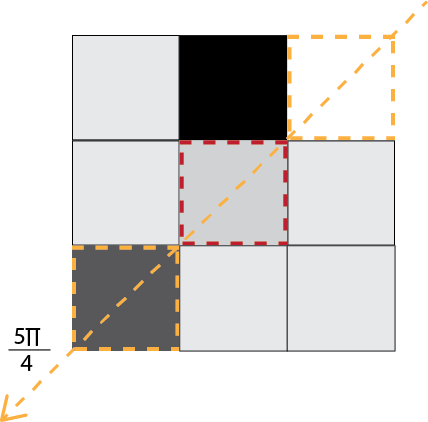
\includegraphics[width=0.9\textwidth]{nms2-before.png}
            \caption{Before NMS}
            \label{fig:nms2-before}
        \end{subfigure}
        \hfill
        \begin{subfigure}[b]{0.40\textwidth}
            \addtocounter{subfigure}{-1}
            \renewcommand\thesubfigure{\alph{subfigure}2}
            \centering
            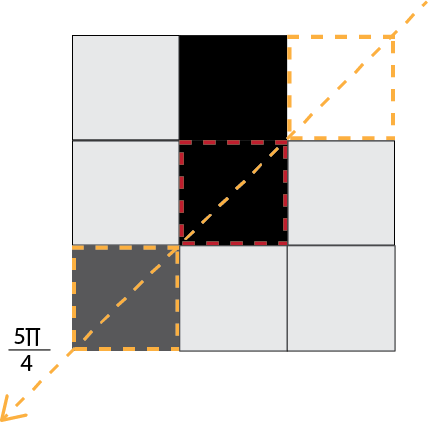
\includegraphics[width=0.9\textwidth]{nms2-after.png}
            \caption{After NMS}
            \label{fig:nms2-after}
        \end{subfigure}
        \addtocounter{subfigure}{-1}
        \caption{Suppression}
        \label{fig:nms2}
    \end{subfigure}
    \caption{Visualization of Non-Maximum Suppression}
    \label{fig:nms-examples}
\end{figure}

The result of applying non-maximum suppression to the gradient magnitude image is shown in \autoref{fig:nms}.

\begin{figure}[ht]
    \centering
    \begin{subfigure}[b]{0.4\textwidth}
        \centering
        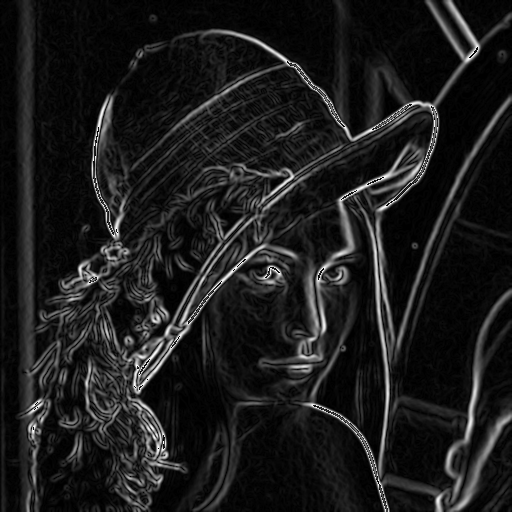
\includegraphics[width=0.9\textwidth]{lenna_4_gradient_magnitude.png}
        \caption{Gradient Magnitude}
        \label{fig:gradient-magnitude-wo-nms}
    \end{subfigure}
    \hfill
    \begin{subfigure}[b]{0.4\textwidth}
        \centering
        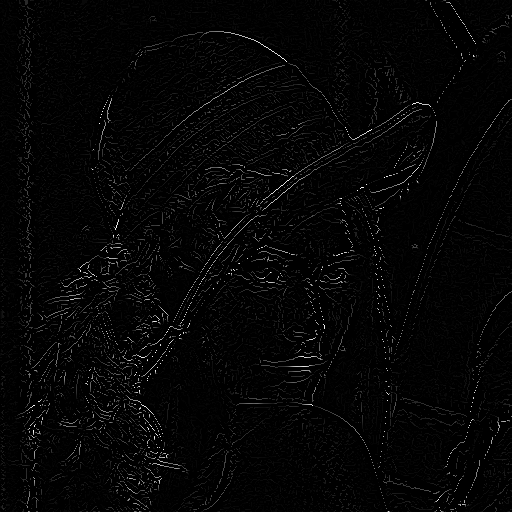
\includegraphics[width=0.9\textwidth]{lenna_6_non_max_suppressed.png}
        \caption{After Non-Maximum Suppression}
        \label{fig:gradient-magnitude-with-nms}
    \end{subfigure}
    \caption{Effect of Non-Maximum Suppression on Gradient Magnitude}
    \label{fig:nms}
\end{figure}